\documentclass[../TDE7_ocrsf.tex]{subfiles}%

\begin{document}
\section[s]"1"{Condition de résonance}
\enonce{%
	\begin{minipage}{0.60\linewidth}
		Le circuit ci-contre est alimenté par une source de tension sinusoïdale de
		f.é.m. $e(t) = E_0 \cos( \wt)$. On s'intéresse à la tension $u(t)$
		aux bornes du résistor et de la capacité montés en parallèle.

		On pose~: $\w_0 =\dfrac{1}{\sqrt{LC}}$, $\xi =
			\dfrac{R}{2}\sqrt{\dfrac{C}{L}}$ et $x = \dfrac{\w}{\w_0}$.
	\end{minipage}
	\hfill
	\begin{minipage}{0.35\linewidth}
		\begin{center}
			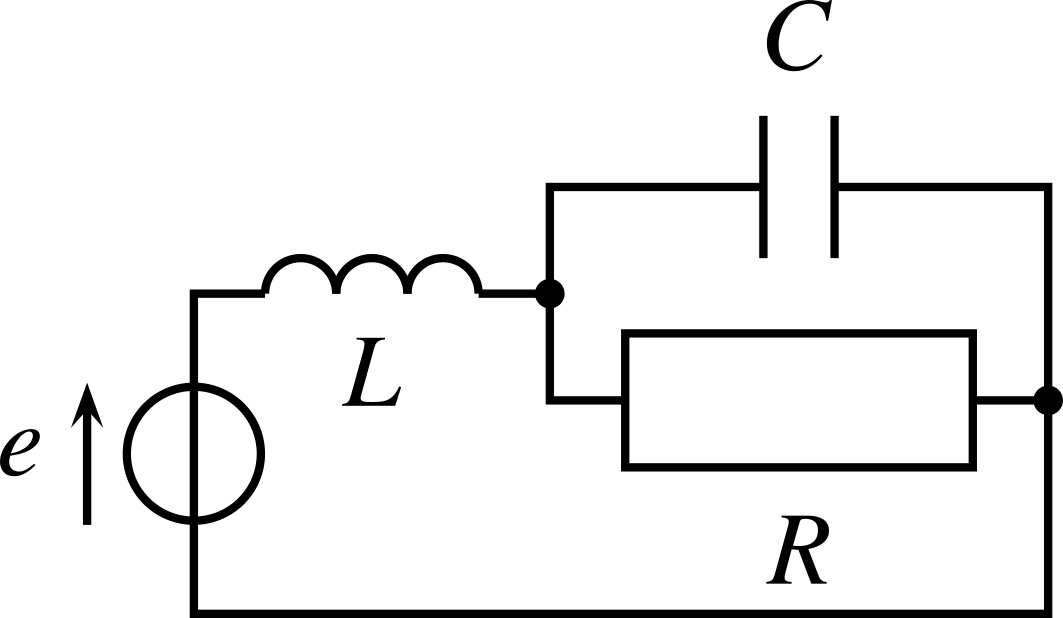
\includegraphics[width=\linewidth]{cond_res}
		\end{center}
	\end{minipage}
}

\QR{%
	Établir l'expression du signal complexe $\xul{u}$ associé à
	$u(t)$ en régime sinusoïdal forcé, en fonction de $E_0$, $x$ et
	$\xi$.
}{%
	Soit $\Zu$ l'impédance équivalent à l'association en parallèle de $R$
	et $C$. On a
	\begin{gather*}
		\Zu = \frac{R/\jcw}{R + 1/\jcw} = \frac{R}{1+\jj RC\w}
	\end{gather*}
	En utilisant un pont diviseur de tension, on trouve
	\begin{gather*}
		\uu = \frac{\Zu}{\Zu + \jlw}\eu
		= \frac{1}{1+\jlw/\Zu}\eu\\
		\Leftrightarrow
		\uu = \frac{\eu}{1+ \jj \frac{L\w}{R} - LC\w^2}
		= \frac{\eu}{1+ 2\jj\xi x - x^2}
	\end{gather*}
}

\QR{%
	Étudier l'existence éventuelle d'une résonance pour la tension
	$u(t)$.
}{%
	L'amplitude réelle est
	\begin{gather*}
		U = \abs{\uu} = \frac{E_0}{\sqrt{(1-x)^2 + (2\xi x)^2}}
	\end{gather*}
	On trouve le maximum de cette amplitude quand le dénominateur est
	\textbf{non nul} et minimal, c'est-à-dire
	\begin{gather*}
		U(\w_r) = U_{\max}
		\Leftrightarrow
		\left( 1 - x^2 \right)^2 + \left(2\xi x\right)^2 \text{minimal}
	\end{gather*}
	Soit $X = x^2$, et $f(X) = \left(1 - X\right)^2 + 4\xi^2X$, la fonction que
	l'on cherche à minimiser~: on cherche donc quand est-ce que sa dérivée est
	nulle, c'est-à-dire
	\begin{gather*}
		f'(X_r) = 0
		\Leftrightarrow
		-2 \left( 1-X_r \right) + 4\xi^2 = 0
		\Leftrightarrow
		X_r-1 = - 2\xi^2
		\Leftrightarrow
		X_r = 1 - 2\xi^2\\
		\Leftrightarrow
		\boxed{
			\w_r = \w_0 \sqrt{1 - 2\xi^2}}
	\end{gather*}
	ce qui n'est défini \textbf{que si} $\xi < \frac{1}{\sqrt{2}}$. Ainsi,
	\begin{itemize}[leftmargin=60pt]
		\item{}[$\mathbf{\xi \geq 1/\sqrt{2}}$] : \textbf{pas de résonance},
		      l'amplitude est maximale pour
		      \[\boxed{\w = 0 \qet U(0) = E_0}\]
		\item{}[$\mathbf{\xi < 1/\sqrt{2}}$] : l'amplitude est maximale pour
		      \[\boxed{\w_r = \w_0 \sqrt{1 - 2\xi^2} < \w_0}\]
	\end{itemize}
}
\end{document}
